\documentclass{article}
\usepackage{graphicx}
\usepackage[margin=1.5cm]{geometry}
\usepackage{amsmath}

\begin{document}

\title{Wednesday Reading Assessment: Unit 6, Circular Motion}
\author{Prof. Jordan C. Hanson}

\maketitle

\section{Memory Bank}

\begin{itemize}
\item $T^2 \propto r^3$ ... Kepler's Third Law
\item Given two planets, we can use this like:
\begin{equation}
\left(\frac{T_2}{T_1}\right)^2 = \left(\frac{r_2}{r_1}\right)^3 \label{eq:orb}
\end{equation}
\end{itemize}

\section{Kepler's Laws}

\begin{enumerate}
\item
\begin{figure}[ht]
\centering
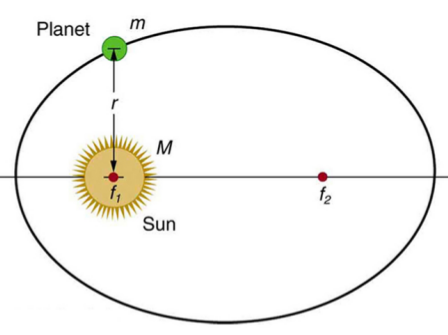
\includegraphics[width=0.35\textwidth]{orbit.png}
\caption{\label{fig:orbit} A planet orbits around the Sun.}
\end{figure}
Suppose we define a unit called an ``Astronomical Unit'' that is equal to $1.496\times 10^8$ km.  This is the distance between the Earth and the Sun.  So we can say that the Earth is 1 AU from the Sun.  It turns out that Venus is 0.72 AU from the Sun (it's closer).  The orbit of the Earth is 1 year.  Let $T_1 = 1$ year, $r_1 = 1.0$ AU for the Earth, and $r_2 = 0.72$ AU for Venus.  Use Eq. \ref{eq:orb}. to find the orbital period of Venus, $T_2$. \\ \vspace{3cm}
\item The orbital period of Jupiter is observed to be 11.8 years.  How far in AU is Jupiter from the Sun?  (\textit{Hint: it's the same procedure as the prior problem using Earth's numbers, but solving for $T_2$}).
\end{enumerate}
\end{document}
